\section{Arkitektur-overvejelser}\label{sec:arkitektur}
For at skabe et overblik over forskellige relationer, attributter og multiplisiteter, 
har gruppen valgt at lave en domænemodel.
Domænemodellen sikrer at gruppen har en repræsentation af de klasser, som skaber det domæne systemet berører.\\

Domænemodellen kan ses på figur (\ref{fig:domain})

\begin{figure}[H]
    \centering
    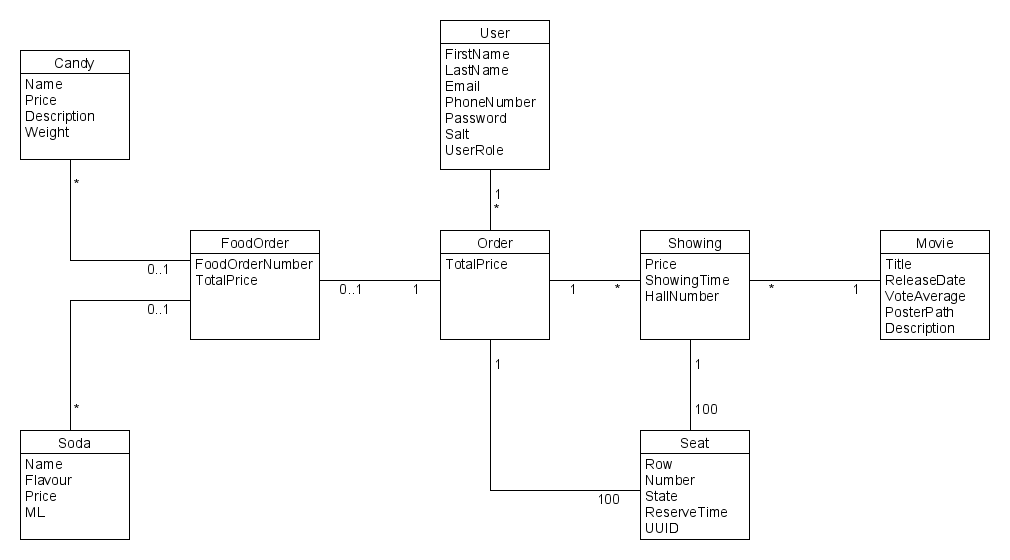
\includegraphics[width=1\textwidth]{figures/Domainmodel.png}
    \caption{Domænemodel}
    \label{fig:domain}
\end{figure}

Domænemodellen er udarbejdet over flere iterationer, og er derfor blevet ændret en del gange.
Venstre side af modellen er ikke blevet implementeret (fra FoodOrder), da gruppen har valgt at fokusere på
en anden user story, nemlig "Create Booking", som resten af domænemodellen beskriver. Dette skyldes at "Create Booking"
giver den største forretningsværdi.

